\documentclass[letter]{article}

\setlength{\pdfpagewidth}{8.5in}
\setlength{\pdfpageheight}{11in}

\usepackage{ijcai13}
\usepackage{amsmath} 
\usepackage{amsfonts}
\usepackage{tikz} % don't have to include
\usepackage{tikz-qtree}
\usepackage[font=small]{subcaption}
\usepackage[font=small]{caption}
\usepackage{dashrule} 
\usetikzlibrary{arrows,automata, positioning, patterns,backgrounds}
\usetikzlibrary{arrows,shapes.gates.logic.US,shapes.gates.logic.IEC,calc}

\usepackage{times}
\pdfinfo{
  /Title (Bootstrap learning via modular concept discovery)
  /Author (Eyal Dechter, Jon Malmaud, Ryan P. Adams, Joshua B. Tenenbaum)
}

\newtheorem{definition}{Definition}
\DeclareMathOperator*{\argmax}{arg\,max} 
\DeclareMathOperator*{\argmin}{arg\,min} 


\title{Bootstrap Learning via Modular Concept Discovery\thanks{We acknowledge the support of ARO MURI W911NF-08-1-0242.}}

\author{Eyal Dechter \\
MIT\\
USA \\
edechter@mit.edu
\And
Jon Malmaud \\
MIT \\ 
USA \\
malmaud@mit.edu
\And 
Ryan~P.  Adams \\
Harvard University\\
USA \\
rpa@seas.harvard.edu
\And
Joshua~B. Tenenbaum \\
MIT\\
USA \\
jbt@mit.edu
}

\begin{document}

\maketitle
\begin{abstract}
 Suppose a learner is faced with a domain of problems about which it
 knows nearly nothing. It does not know the distribution of problems,
 the space of solutions is not smooth, and the reward signal is
 uninformative, providing perhaps a few bits of information but not
 enough to steer the learner effectively. How can such a learner ever
 get off the ground? A common intuition is that if the solutions to
 these problems share a common structure, and the learner can solve
 some simple problems by brute force, it should be able to extract
 useful components from these solutions and, by composing them,
 explore the solution space more efficiently. Here, we formalize this
 intuition, where the solution space is that of typed functional
 programs and the gained information is stored as a stochastic grammar
 over programs. We propose an iterative procedure for exploring such
 spaces: in the first step of each iteration, the learner explores a
 finite subset of the domain, guided by a stochastic grammar; in the
 second step, the learner compresses the successful solutions from the
 first step to estimate a new stochastic grammar. We test this
 procedure on symbolic regression and Boolean circuit learning and
 show that the learner discovers modular concepts for these
 domains. Whereas the learner is able to solve almost none of the
 posed problems in the procedure's first iteration, it rapidly becomes
 able to solve a large number by gaining abstract knowledge of the
 structure of the solution space.
\end{abstract}

\section{Introduction}

Imagine that you know nothing about electronics but are supplied with
a collection of circuit elements and asked to build a number of useful
digital devices, such as an adder, a flip-flop, a counter, a
multiplexer, and so on.  Your initial attempts will probably be
uniformly ineffective.  If your only feedback is based on success or
failure, you may have trouble learning anything.  If, on the other
hand, you already know the basics of circuit design, you are far more
likely to generate some devices that are at least somewhat successful.
In this case, with feedback you can improve your designs and your
design skills.

This example illustrates the central ``bootstrapping'' challenge for
attempts to create intelligent agents without building in vast amounts
of pre-specified domain knowledge.  Learning from experience is
typically most effective in a system that already knows much of what
it needs to know, because mistakes are most informative.  In a system
that knows almost nothing, where most problem solving attempts
entirely miss their mark, failures are unlikely to shed light on what
will work and what will not.  Uninformative solutions vastly outnumber
the rest, and an uninformed agent has no way to know which solutions
will be informative and which will not.  If it is harder to learn the
less an agent knows, how can a learner who knows almost nothing about
a domain ever get off the ground?

Here we propose an answer to this challenge, based on an approach to
discovering new and increasingly sophisticated concepts that build
modularly on previously learned, simpler concepts.  Like many problems
in AI, the bootstrapping challenge and its solution can be cast in
terms of search.  In our circuit-building scenario, the goal is to find
circuit wiring procedures that maximize certain criteria.  Search
algorithm typically aim to exploit local or topological structure in
the search space -- here the space of all circuit-wiring procedures.
For example, local search algorithms move from one candidate solution
to a neighboring one. Heuristic search techniques take advantage of
topological structure to prune off large parts of the search space.
This structure derives from domain-specific knowledge.  In local
search, domain knowledge provides the similarity metric between
solutions; in heuristic search it provides the heuristic.  Here we ask
how to bootstrap domain-specific knowledge by extracting search
structure from the space of possible solutions, by attempting to solve
multiple related problems in a given domain at once.

Our approach is motivated by the observation that many interesting
problems –- such as discovering scientific theories, designing new
technologies, learning a skill such as playing an instrument or
cooking –- have solutions that are naturally specified as programs.
Our proposed solution is inspired by the programmer who, having found
various subroutines that can be reused to solve similar simple tasks,
creates a function library to help manage the complexity of larger
projects. The E.C. algorithm, which we introduce here, builds a
library of reusable program components and places a distribution over
these, effectively learning from simple tasks a search space structure
that enables it to solve more complex tasks.

In this work, we try to see how far this idea of reusable function
definition can get us. We ask the following question: can an AI system
discover the structure latent in the solutions to multiple related
problems and thereby bootstrap effective exploration of the search
space? Can discovering modular program components transform a problem
from one in which search is intractable into a problem in which it
becomes increasingly feasible with experience?

Concretely, the E.C. algorithm works as follows. It begins with a small
library of program primitives and a distribution over programs
synthesized from this library. In each iteration, it generates
programs in order of highest probability according to the library
learned in the previous iteration. From the discovered solutions, it
finds new reusable functions that compress these solutions, and it
re-estimates the distribution over programs by weighting these new
functions according to their frequencies. In using compression as a
guide to the choice of representation, we instantiate the idea that
good representations are those which minimize the description length
of typical elements in the domain.

We show that this iterative approach allows us to achieve very high
performance in tasks where just searching according to the initial
distribution over program primitives clearly fails.


\section{Related Work}
The idea of discovering and using reusable subcomponents is part of an
old tradition in AI. For instance, it is one of the central themes in
Herb Simon's ``The Sciences of the
Artificial''~\shortcite{simon1996sciences}. Rendell's ``Substantial
Constructive Induction Using Layered Information Compression:
Tractable Feature Formation in Search'' presented within a classical
search paradigm the idea that compression provides a heuristic for
constructing good
representations~\shortcite{DBLP:conf/ijcai/Rendell85}. Within the
Inductive Logic Programming (ILP) literature, researchers have
explored ``Constructive Induction,'' generating new and reusable logic
programming terms~\cite{DBLP:conf/ijcai/Muggleton87}. Later, predicate
invention was also applied in the multitask
setting~\cite{DBLP:conf/ilp/KhanMP98}. We apply these ideas to
learning functional programs and believe that the modularity and
compositionality afforded by this representation is necessary for
these ideas to be successful.


Genetic programming
(GP)~\cite{DBLP:conf/foga/Koza92,DBLP:conf/ices/KozaBAK96} has
tackled the problem of program learning and has explored the notion
that reusable functions are helpful. This work relies, however, on
stochastic local search over the space of programs, and automatically
discovering useful subroutines is seen as a helpful heuristic. More
recently, Liang et al.~\shortcite{liang10programs} used a stochastic
grammar over combinatory logic to induce shared structure in
multi-task program induction problems. We find this latter
representation compelling and use it here, but we see both this and
genetic programming as tackling the question of how to benefit from
shared structure in situations where local search might be successful
on its own. Such problems rely on domain knowledge -- whether in the
form of a fitness function or a likelihood function -- to provide
local structure to the search space.

But, as mentioned before, the problems we want AI systems to solve
often lack this kind of built in structure. Here we attempt to learn
functional programs to solve those kinds of problems.  \\

%% AI and machine learning algorithms commonly take advantage of the
%% relationship between a performance metric (error, reward, fitness,
%% etc.) and the local or topological structure of the solution
%% space. Whether in discrete or continuous domains, the key is to design
%% such a relationship and write a algorithm that either moves in good
%% directions or prunes off large parts of the solution space. Whether or
%% not such a relationship exists depends on the representation, and much
%% work has gone into finding good representations for problem
%% solving. Recent work, especially in machine learning, has focused on
%% ``feature learning,'' with the explicit aim of discovered good
%% representational building blocks in vector-valued solutions spaces.

%% Many of the most natural solution representations for intelligent
%% agents, however, are not naturally expressed as vector-valued
%% spaces. Consider the problems of discovering scientific theories,
%% inventing new technologies, communicating with others, or executing a
%% complex motor routine (such as dancing or playing an instrument). The
%% solutions to these problems are most naturally expressed as programs,
%% that is, as the composition of modular components whose semantics are
%% determined by the actions of one component on another.

%% How can we learn good solution representations for these kinds of
%% tasks without building in the kind of domain knowledge that gives rise
%% to a useful relationship between representation and performance? How
%% can we get traction on a set of problems when small tweaks to
%% solutions give rise to wildly varying performances in an unpredictable
%% manner, or when, for most problems, most of the solutions fail in a
%% uniformly bad way? 

%% A popular idea is that good representations are those that encode the
%% data space in an efficient way, that is, that enable compression of
%% the data~\cite{}. For program representations, this most naturally
%% corresponds to defining reusable components so that the total number
%% of unique expressions for a set of solutions is minimized (i.e., this
%% is directly akin to the subroutine libraries programmers use to manage
%% the complexity of their code). 

%% In this work, we try to see how far reusable subroutine definition can
%% get us on its own. Our question is, Can discovering modular components
%% transform a problem from one in which brute-force search will not work
%% to a problem in which it does? 

%% To emphasize an impoverished relationship between reward signals and
%% program representations, we make our tasks all-or-none: a solution
%% either solves the problem or it does not, and partial solutions do not
%% get any credit. 

%% The intuitive approach to applying this idea is simple: if solutions
%% to problems in the domain share common structure, and there exist
%% problems whose solutions are simple enough to find by brute force,
%% then we should be able to extract a distribution over solution
%% subcomponents from these simple cases that allows us to run subsequent
%% searches more efficiently. 

%% More concretely, our algorithm works as follows: each iteration, it
%% first generates programs in order of highest probability according to
%% a subroutine distribution learned in the previous iteration. From the
%% discovered solutions, it finds new reusable subroutines that compress
%% these solutions and estimates their probabilities.

%% We show that this iterative approach allows us to achieve very high
%% performance in tasks where just searching according to the initial
%% distribution over program primitives clearly fails.



%%  \hline

%% AI and machine learning algorithms commonly take advantage of the idea
%% that local structure in the solution space is related to local
%% structure in the outcome. In continuous domains, learning algorithms
%% algorithms use error gradients to guide search. In discrete domains,
%% whether in heuristic or local search paradigms, knowledge about the
%% solution space topology and its relation to reward and cost metrics
%% enables pruning, reasoning, and moving in the solution space more
%% efficiently. However, choosing the representations that have
%% beneficial structural properties requires a lot of general and domain
%% knowledge, and this what researchers do and what they cannot leave up
%% to their algorithms.

%% What is a good strategy for an agent when its representation of the
%% solution space is not smooth with respect to the outcome? Many hard
%% learning problems have this property, especially those in which the
%% solution space is most naturally represented as a set of
%% programs. Consider the problems of discovering scientific theories,
%% inventing new technologies, learning to cook, or learning to
%% communicate. These are problems in which 1) solutions are best
%% described as programs (i.e. compositions of modular subroutines at
%% various levels of abstraction), 2) most of the solution space is bad
%% in a relatively uninformative way (i.e. it just doesn't work), and
%% thus 3) outcomes are not informative about how you are doing unless
%% you are already quite close to a solution.

%% Intuitively, the way to solve such problems is to find solutions to
%% simple cases in the domain and extract conceptual building blocks that
%% can be composed to scale up to complex cases. With experience, the
%% agent may be able to discover local structure in the solution space,
%% and utilize more traditional AI and machine learning techniques. In
%% this work, we will be focusing on the first phase of this learning
%% problem.

%% %% Of course, every learner 

%% %% Choosing the wrong representation, in
%% %% which local structure is not apparent, is often the difference between
%% %% a successful learner and an unsuccessful one. In many respects, this
%% %% may be the kind of situation that adult humans face when confronting
%% %% new domains: we have a lot of general knowledge of successful
%% %% representations, useful strategies, etc.

%% %% But suppose that you have very little knowledge of a domain. Your
%% %% initial representation of the domain is poor: ``nearby'' points in the
%% %% solutions space elicit wildly different outcomes in unpredictable
%% %% ways. Or perhaps nearby points elicit the same outcome and its not a
%% %% good one, so you don't know which way to go. Many learning problems,
%% %% especially those whose solutions are best described as programs, have
%% %% these qualities: imagine learning to synthesize new sentences





%% %% teness. We choose the representations our learners use
%% %% and these representations generally Imagine you are trying to learn to
%% %% bake via trial and error. You know what kind of ingredients are used
%% %% in baking (flour, water, butter, sugar, yeast, baking soda, etc.) and
%% %% you know a bit about how to combine these ingredient (mix, whisk,
%% %% etc.) and how to apply heat (oven). But baking is a notoriously
%% %% fragile process: ratios of ingredients, the order of mixing, cooking
%% %% temperatures, resting times, all make a huge difference, and the
%% %% outcome of the baking process is mostly all or none. Either the
%% %% outcome is what you expected or quite unlike it. Even if you do create
%% %% something similar to your intent, it is difficult to assign blame for
%% %% the outcome to any one step or decision along the way.

%% %% Many difficult learning problems have this structure -- learning
%% %% language, developing technologies and scientific theories, learning to
%% %% play instruments or execute other complex motor patterns. These are
%% %% problems in which 1) there is a large set of similar tasks; 2) their
%% %% solutions are best described as programs; 3) the solution space is
%% %% not smooth with respect to the outcome; 4) and the outcome is generally
%% %% uninformative unless you are already pretty close to a solution.

%% %% Of course, knowledge is not acquired wholly by trial and error. But in
%% %% many domains, there is at least initially such a period of ignorance,
%% %% and the question we are trying to tackle here is how you ever get off
%% %% the ground.


%% I need help here. 

%% %% Let a \emph{task} be a function $t : \mathcal{L} \rightarrow \{0,
%% %% 1\}$, where $\mathcal{L}$ is the set of all expressions in our
%% %% representation language. We say that $e \in \mathcal{L}$ \emph{solves}
%% %% task $t$ if $t(e) = 1$. Our goal is to solve as many tasks as
%% %% possible, as efficiently as possible. That is, suppose that there is a
%% %% distribution over tasks $t \sim  p_t(\cdot)$, we would like an ordering $O
%% %% = e_1, \dots $ on expressions in $\mathcal{L}$ such that if $p_t(t_1)
%% %% > p_t(t_2)$ then the first expression in $O$ to solve $t_1$ comes
%% %% before the first expression in $O$ to solve $t_2$.

%% %% We motivate a solution to this problem by considering a heirarchical
%% %% Bayesian formulation of the task distribution. Suppose we believe that
%% %% there is some underlying structure to $p_t(\cdot)$ that is explained by
%% %% the fact that for each task $t$ there is a latent expressions $e \in
%% %% \mathcal{L}$ drawn from a stochastic grammar $\mathcal{G}$ and that 

%% %% \begin{align}
%% %% e &\sim p_\mathcal{L}(\cdot) = \mathcal{G}\\
%% %% t | e &\sim \text{U}\{ \text{tasks solved by }e\}.
%% %% \end{align}

%% %% Then $p_t(t) = \sum_{e_j \in \mathcal{L} \text{ s.t. } t(e_j) = 1}
%% %% p_\mathcal{L}(e_j)$. If we make the assumption that for the set $E$ of
%% %% expressions in this sum, there is some expression $e^*$ such that
%% %% $p_\mathcal{L}(e^*) >> p_\mathcal{L}(e), e \neq e^*$, then we have, approximately, 
%% %% \[ p_t(t) \propto} p_\mathcal{L}(e^*). \] 

%% %% This suggests a way to find the ordering $O$: infer a stochastic
%% %% grammar $G$, under the assumption that $G$ favors one solution to a
%% %% given task over any other, and order the elements of $\mathcal{L}$
%% %% according to $G$.

%% %% Thus, our basic procedure will be to search for a single ``good''
%% %% solution for as many tasks as we can, and to use those solutions to
%% %% estimate a stochastic grammar. Our search will be performed in the
%% %% order of the most recently inferred grammar. So as our ordering
%% %% becomes more efficient and we can solve more tasks, we learn better
%% %% stochastic grammars.

%% %% Formally then, our goal is to solve the following minimal feedback
%% %% multi-task program induction problem: suppose we are given set of
%% %% \emph{tasks} $T=\{t_k\}_{k=1}^K$ where each task is a function $t_i :
%% %% \mathcal{L} \rightarrow \{0, 1\}$, where $\mathcal{L}$ is the set of
%% %% programs in our language.  We say that $ p \in \mathcal{L}$
%% %% \emph{solves} $t_i$ if $ t_i(p) = 1$. Our goal is to find a set of
%% %% solutions $X = \{x_k\}_{k=1}^k \subset \mathcal{L}$ such that

%% %% \[
%% %% X = \argmax_{x_1, \dots, x_K \in L} \sum_k t_k(x_k).
%% %% \]

%% Based on the motivation set out above, we present an iterative
%% strategy. Given a stochastic grammar $\mathcal{G}$ which defines a
%% distribution over the primitives from $\mathcal{L}$ and a integer
%% \emph{frontier size} $N$, we perform two steps in each iteration.  In
%% the first step, we explore the $N$ highest probability programs
%% according to $\mathcal{G}$. In the second step, we compress the
%% programs that solve any of our tasks, and we use that compression to
%% define a new grammar. Repeating these two steps, we effectively
%% reparameterize our search space to include programs that are more likely
%% to be solutions to our tasks. 

The remainder of this paper will include two major sections. In the
first, we describe in detail the E.C. algorithm and design choices we
make in implementing it. We will then present results from two
experiments in the domains of symbolic regression and Boolean
function learning.

%% \section{}
%% Let $\mathcal{F}$ be a family of distributions over $\mathcal{L}$ such
%% that for any $\mathcal{D} \in \mathcal{F}$ we can a) evaluate the
%% probability of program $p$, $P_D(p)$, and we can b) enumerate elements
%% from $D$ in descending order. 


%%  To motivate a solution to our problem, we begin with the hierarchical
%% Bayesian formulation of multi-task program induction found in Liang et
%% al.~\cite{liang10programs}. The general idea there is to estimate
%% solution programs for a set of related problems by inferring the posterior
%% distribution over solutions under the assumption that all the solution
%% programs are generated from a common latent stochastic grammar. By
%% jointly inferring solutions and the latent grammar, we find a set of
%% solutions that favors reuse of subcomponents.

%% While this framework is appealing in its elegance and Bayesian
%% interpretation, it cannot be straightforwardly adapted to the
%% situation we are considering here because their proposed MCMC
%% algorithm relies on a local log-likelihood signal, the very kind that
%% we are assuming we do not have access to.

%% To begin, we provide a high level overview of the algorithm and the
%% problem that it solves. The problem setup requires a representation
%% language for programs and a family of distributions over expressions
%% in that language, but we leave these details for the following section

\section{Extracting Concepts from Programs}

Our goal is to solve the following minimal feedback multi-task program
induction problem: suppose we are given a set of \textbf{tasks}
$T=\{t_k\}_{k=1}^K$ where each task is a function \mbox{$t_k : \mathcal{L}
\rightarrow \{0, 1\}$} and where $\mathcal{L}$ is the set of
expressions in our language.  We say that expression $ e \in
\mathcal{L}$ \textbf{solves} $t_k$ if $ t_k(e) = 1$. Our goal is to
solve as many of the tasks in $T$ as we can. 

We propose the \textbf{E.C. algorithm}, an iterative procedure to solve this
problem. It will be useful in presenting the algorithm to define the
following terminology: a \textbf{frontier} is the finite set of
expressions that the algorithm considers in any one iteration. The
\textbf{frontier size} $N$ is the pre-specified number of elements in
the frontier. We will say that a task is \textbf{hit} by the frontier
if there is a expression in the frontier that solves it.

The E.C. algorithm maintains a distribution $\mathcal{D}$ over
expressions in $\mathcal{L}$. At each iteration, it
\begin{enumerate}
\item \textbf{explores} the frontier -- enumerating the $N$ most probable expressions
  from the current distribution $\mathcal{D}$ -- and
\item \textbf{compresses} the hit tasks in the frontier to estimate a new
  distribution.
\end{enumerate}

\subsection{Representing Typed Functional Programs as Binary Trees}

Following~\cite{liang10programs} and~\cite{briggs2006functional}, we use a
simply typed combinatory logic -- a variable-free subset of the
polymorphic simply-typed lambda calculus~\cite{Pierce_2002} -- as our
program representation language. In short, the combinatory logic
introduces a \emph{basis} of several primitive \emph{combinators} such
that any function can be written as applications of the basis
combinators. Some common basis combinators are defined as follows:
\begin{align}
\mathbf{I}\; x &\rightarrow  x & \text{ (identity) }\\
\mathbf{S}\; f\; g\; x\; &\rightarrow (f\; x)\; (g\; x)\\ 
\mathbf{C}\; f\; g\; x\; &\rightarrow (f\; x)\; g  \\ 
\mathbf{B}\; f\; g\; x\; &\rightarrow f\; (g\; x) & \text{ (composition) }
\end{align}

The basis combinators are theoretically enough to express any Turing
computable function, but we will assume that our language has a
variety of primitives and, together with the basis combinators, we
call these the \textbf{primitive combinators}. Note that by default we consider
all primitives to be in their ``curried'' form (e.g. a function like
``+'' adds two numbers $x$ and $y$ by being first applied to $x$,
returning the function $(+\;x)$ and then being applied to $y$,
returning $(+\,x\,y)$\;).

The basis combinators can themselves be expressed in the lambda
calculus (with definitions following directly from the equations
above). The lambda calculus has two basic operations -- application
and abstraction -- but in using the
combinatory logic we sequester uses of the abstraction operation
inside the combinators. In doing so, we have replaced the variable
binding of the $\lambda$ operator with the variable \emph{routing} of
these basis combinators. Our representation thus becomes
variable-free. See \cite{liang10programs} for a more
detailed discussion of this routing interpretation.

Using combinatory logic is very convenient for program
synthesis~\cite{briggs2006functional}: since every expression is the
application of one expression to another -- with this recursion
bottoming out at the primitive combinators -- each program is a binary
tree. Most importantly, any subtree is itself a well-formed
expression; this is not the case in the lambda calculus, since
abstraction introduces long range dependencies between the $\lambda$
operator and the variables to which that operator refers. In the
lambda calculus, then, a subtree might have free variables, not bound
to any enclosing $\lambda$.

As a simple example of our representation, consider the squaring
function $\lambda x. * x\; x $. Using two of the basis combinators
above, we can write the squaring function in combinatory logic as $S\; *\;
I$ (taking $*$ as a primitive), where application associates to the
left, so we drop the parentheses. When we apply this combinator to a
value $x$, the action of the combinator is defined as $S \;*\; I\;
x~\rightarrow~(*\; x)\; (I\; x)~\rightarrow *\; x \; x$.

We can extend this representation with a simple polymorphic type
system~\cite{Pierce_2002}. In this representation, a type is either a
type primitive (e.g. reals, integers, Booleans, etc.), a type variable
(e.g. $\sigma$), or a function type $ \tau_1 \rightarrow \tau_2$ of
functions from source type $\tau_1$ to target type $\tau_2$. Any combinator
can be represented as a binary tree~(Figure~\ref{fig:clbintree}) whose
leaves are typed primitive combinators and whose interior nodes
represent typed applications of combinators (we annotate interior
nodes with their types).

\begin{figure}
%%  \centering
  \begin{subfigure}[Before]{0.45\linewidth}
    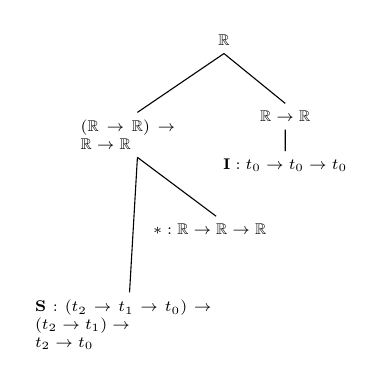
\begin{tikzpicture}[scale=.8,
        transform shape, level/.style={sibling distance=5mm/#1, font=\scriptsize}
        ]
      \node [font=\scriptsize] (top) {$\mathbb{R}$}
      child {node [above=.3cm, left=.1cm, text width=1.8cm] (a) {$(\mathbb{R} \rightarrow \mathbb{R}) \rightarrow \mathbb{R} 
          \rightarrow \mathbb{R}$}
        child {node [left=.5cm, below=1cm, text width=3.0cm] 
          {$ \mathbf{S} : (t_2 \rightarrow t_1 \rightarrow t_0)  \rightarrow (t_2 \rightarrow t_1) 
            \rightarrow$ \\ $t_2 \rightarrow t_0$}}
        child {node [right=0cm, text width=2cm] {$ \mathbf{*}: \mathbb{R} \rightarrow \mathbb{R} \rightarrow \mathbb{R}$}}
      }
      child {node [below right=-.5cm and .2cm] (b) {$\mathbb{R} \rightarrow \mathbb{R}$}
        child {node [above=.5cm] {$ \mathbf{I}: t_0 \rightarrow t_0 \rightarrow t_0$}}
      };
    \end{tikzpicture}
    \caption{    \label{fig:clbintree}}
  \end{subfigure}
  \begin{subfigure}[After]{0.5\linewidth}
    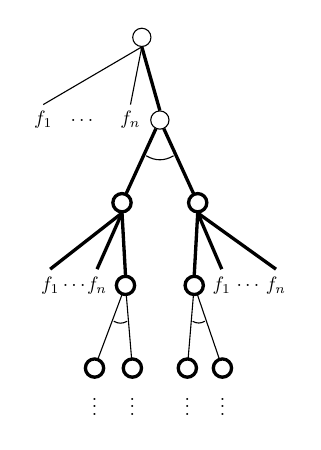
\begin{tikzpicture}[scale=.7, transform shape, 
        level/.style={sibling distance=10mm/#1},
        every edge/.style={draw, thin}
      ]
      \node [circle,draw] (a) {}
      child {node [left=0cm] (b) {$f_1$}}
      child {node [left=.2cm] (c) {\dots} edge from parent[draw=none] }
      child {node [left=.4cm] (e) {$f_n$}}
      child {node [circle,draw, left=1cm] (d) {} edge from parent[very thick]
        child {node [circle, draw, left=.25cm] (l) {} edge from parent[draw=none]
          child {node [left=.5cm] (b) {$f_1$}} 
          child {node [left=.3cm] (c) {\dots} edge from parent[draw=none] }
          child {node [left=.3cm] (e) {$f_n$} edge from parent[very thick]}
          child {node [circle, draw, left=.25cm] (and2) {}
            child {node [circle, draw, left=.25cm](l2) {} edge from parent[draw=none] 
              child {node [above=.5cm] {\vdots} edge from parent[draw=none]}
            }
            child {node [circle, draw] (r2)  {} edge from parent[draw=none] 
              child {node [above=.5cm] {\vdots} edge from parent[draw=none]}
            }
          }
        }
        child {node [circle, draw, right=.25cm] (r) {} edge from parent[draw=none]
          child {node [circle, draw, right=.25cm] (and3) {}
            child {node [circle, draw ](l3) {} edge from parent[draw=none] 
              child {node [above=.5cm] {\vdots} edge from parent[draw=none]}
            }
            child {node [circle, draw, right=.2cm ] (r3)  {} edge from parent[draw=none] 
              child {node [above=.5cm] {\vdots} edge from parent[draw=none]}
            }
          }
          child {node [right=.3cm] (b) {$f_1$} edge from parent[very thick]} 
          child {node [right=.4cm] (c) {\dots} edge from parent[draw=none] }
          child {node [right=.6cm] (e) {$f_n$}}
        }
      };
      
      \path (d)  edge[very thick]  node[inner sep=0mm,pos=.4] (a1) {} node {} (l);
      \path (d)  edge[very thick]  node[inner sep=0mm,pos=.4] (b1) {} node {} (r);
      \path (a1) edge[bend right] (b1) ;

      \path (and2)  edge node[inner sep=0mm,pos=.4] (t0) {} node {} (l2);
      \path (and2)  edge node[inner sep=0mm,pos=.4] (k0) {} node {} (r2);
      \path (t0) edge[bend right] (k0) ;

      \path (and3)  edge node[inner sep=0mm,pos=.4] (t1) {} node {} (l3);
      \path (and3)  edge node[inner sep=0mm,pos=.4] (k1) {} node {} (r3);
      \path (t1) edge[bend right] (k1) ;
    \end{tikzpicture}
    \caption{  \label{fig:andor}}
    \end{subfigure}
  \caption{(a) The typed combinator $S * I$ ($f(x)=x^2$ over real values ($\mathbb{R}$)) represented as a
    binary tree. (b) The space of all typed combinators represented as an
    infinitely deep AND/OR tree.}

\end{figure}

\subsection{A Stochastic Grammar over Programs}
\label{sec:stochgrammar}

We specify a distribution $\mathcal{D}$ over expressions in
$\mathcal{L}$ as a stochastic
grammar~\cite{feldman1969grammatical}. Many stochastic grammars have
the desirable property that the probability of an expression is the
product of the probabilities of its subcomponents. The distribution we
specify will be a simple version of this, in which the
probability of an expression is the product of the probability of its
leaves.

Let ${C = c_1, \dots, c_N }$ be the primitive combinators in
$\mathcal{L}$. ${ \mathcal{D}=p_1, \dots, p_N }$ will associate with
each primitive combinator $c_i$ a prior probability $p_i$,
$0~\leq~p_i~\leq~1, \sum_i~p_i~=~1 $. The probability of a leaf with
primitive combinator $c_i$ will depend on which other primitive
combinators could have been chosen in its place. This set will depend
on the type that was requested by the parent of this leaf when the
leaf's primitive was chosen; we call this type the \emph{requesting}
type of the leaf. For example, suppose that we have the primitive
$(+1)$ of type $Int \rightarrow Int$ and the primitive $NOT$ of type
$Bool \rightarrow Bool$. If the requesting type is $\sigma \rightarrow
Int$, then we can only use $(+1)$, but if the requesting type is
$\sigma \rightarrow \sigma$ then we could use either $(+1)$ or
$NOT$. We define $C_\tau$ for any type $\tau$ to be the set of
primitive combinators in $C$ that are consistent with $\tau$, that is,
whose types \emph{unify} with $\tau$ (we use unification according to
the standard type theory presentation~\cite{Pierce_2002}).

Let $C_e$ be the set of primitive combinators in the leaves of
expressions $e$. We define the probability of an expression ${e \in
  \mathcal{L}}$ to be ${ p(e)~=~\prod_{c \in C_e} p(c | \tau(c)) }$
where $p(c | \tau(c))$ is the probability of using primitive $c$ when
the requesting type is $\tau(c)$. In turn, we define the conditional
probability for each combinator $c_n$ to be $p(c_n| \tau(c_n)) \propto
\frac{p_n}{\sum_{c_j \in C_{\tau(c_n)}} p_j}$.  That is, $p(c_n | \tau(c_n)$ is
proportional to the probability of sampling $c_n$ from the multinomial
distribution defined by the $p_n$'s, conditioned on the requesting
type, with the constant of proportionality chosen to ensure that the
sum over the probabilities of all expressions converges to a finite
value (so that the distribution over expressions is proper). For
binary trees, this is true whenever the constant of proportionality is
less than~$\frac{1}{4}$\footnote{The probability mass $M_d$ of all
  expressions of depth less than or equal to $d$ can be written with
  the recurrence relation $M_d \leq M_{d-1}^2 + M_1$. This has an
  asymptotic fixed point, as $d \rightarrow \infty$ if $x = x^2 + M_1$
  has a solution, which is true if $M_1~\leq~1/4$.}.

Now suppose that we have a set of expressions $\mathcal{E}$, and we
wish to estimate the maximum likelihood values of the $p_n$'s. If the
choice of primitive at each leaf were not conditioned on the
requesting type, we could just count all occurrences of each primitive
in our expression set, and this would be proportional to the maximum
likelihood estimate. This is the ML estimator for a multinomial
distribution. However, the fact that we condition on the requesting
type makes this a considerably more difficult optimization task. One
of the simplest approximations we can make is to calculate the
frequency with which each primitive combinator appears in
$\mathcal{E}$ when the requesting type is such that it could have
been chosen. This is a straightforward calculation, and
we use it for its convenience, finding that our empirical results
justify its use. Future inquiry will be needed to determine to what
extent a more accurate estimator can improve these results.

\subsection{Best-first Enumeration of Programs}
In order to explore the frontier of most promising programs, we need a
procedure that enumerates the $N$ most probable expressions. There has
been recent interest in this problem, most of it focused on
enumerating the shortest program satisfying some
criterion~\cite{DBLP:conf/sfp/Katayama05,DBLP:conf/aaip/YakushevJ09}. Our approach is to formulate the
problem as a best-first exploration of an AND/OR tree
(Figure~\ref{fig:andor})~\cite{nilsson1982principles,DBLP:journals/cacm/Hall73}. In
words, the enumeration procedure is best described by the following
recursion: every program is either a primitive combinator OR it is a
left child program applied to a right child program (that is, a left
child AND a right child).

This can framed as the following AND/OR tree $\mathcal{G}$. Suppose we
want a program of type $\tau$. The root of $\mathcal{G}$ is an OR node of
type $\tau$. Its children are elements in $C_\tau$ (defined in the previous
section) and one AND node of type $\tau$ with two children. Each child of
an AND node has the same structure as the root node, with modified
types: the type of its left child is $\sigma \rightarrow \tau$ (where $\sigma$ is
a fresh type variable). Since the type of the right child is
constrained by the subtree rooted at the left child, we always expand
the left child first. Once we have a complete left child program, we
can use its target type as the type of the right child.

Recall that a valid partial solution $\mathcal{H}$ is a subtree of
$\mathcal{G}$ satisfying the following properties: the root of
$\mathcal{H}$ is the root of $\mathcal{G}$ and any OR node in
$\mathcal{H}$ has at most one child. $\mathcal{H}$ is a complete
solution (and thus a complete expression) if it is a partial solution
whose leaves are leaves of $\mathcal{G}$, if each OR node in
$\mathcal{H}$ has exactly one child, and if each AND node in
$\mathcal{H}$ is connected to all of that node's children in
$\mathcal{G}$.

The value of a partial solution $\mathcal{H}$ is calculated by summing
the value of its leaves, where each such value is the log of the
probability assigned to that leaf in
Section~\ref{sec:stochgrammar}. If a leaf of $\mathcal{H}$ is a leaf
of $\mathcal{G}$ then either it is an AND node, to which we assign a
value of 0, or it corresponds to some primitive combinator $c_n$ in
the library and is the child of some typed OR node with type $\tau$. We
assign it a value of $\log{p(c_n | \tau)}$. If a leaf $v$ of
$\mathcal{H}$ is an OR node, then the value of any extension of it to
a complete solution is at most $log(1/4)$. Thus, we have defined a
value for partial solutions that upper bounds the value of any of its
extensions.

Our best-first policy is to expand the next partial solution
with the highest value. If a partial solution has multiple leaves that
are not primitive combinators, we expand the left most one first,
since it is the choice of left combinator that defines the type of its
right combinator in an application pair. That is, the parent node
applies its constraint on valid solutions via the left child, not the
right child. We want to apply constraints as early as possible, so
expanding left child first prunes more partial solutions.

\subsection{Finding the Most Compressive Set of Solutions}

Having enumerated the frontier, we want to assign solutions
to hit tasks such that this set is maximally compressible. This will
promote reusable modular subtrees. 

A natural metric for the compressibility of a set of binary trees is
the number of unique subtrees (counting leaves) that this set
contains. As an example of this, suppose we have six tasks
whose solutions are integers $4^2, 5^2, 6^2, 7^2$, and $8^2$, and
suppose our frontier contains the $10$ expressions:
\vspace{-.3cm}
\captionsetup[subfigure]{labelformat=empty} 
\begin{figure}[h!]
   \begin{subfigure}{.17\linewidth}
     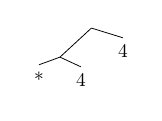
\begin{tikzpicture}[scale=.7, background rectangle/.style={fill=lightgray}] 
       \tikzset{level distance=15pt, sibling distance=10pt}
       \Tree [[  * 4 ] 4 ]
     \end{tikzpicture}
  \end{subfigure}
  \begin{subfigure}{.17\linewidth}
     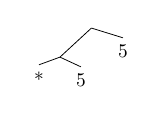
\begin{tikzpicture}[scale=.7]
       \tikzset{level distance=15pt, sibling distance=10pt}
       \Tree [[  * 5 ] 5 ]
     \end{tikzpicture}
  \end{subfigure}
   \begin{subfigure}{.17\linewidth}
     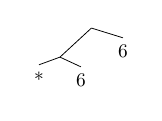
\begin{tikzpicture} [scale=.7]
       \tikzset{level distance=15pt, sibling distance=10pt}
       \Tree [[  * 6 ] 6 ]
     \end{tikzpicture}
  \end{subfigure}
   \begin{subfigure}{.17\linewidth}
     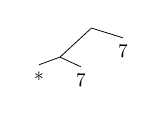
\begin{tikzpicture}[scale=.7] 
       \tikzset{level distance=15pt, sibling distance=10pt}
       \Tree [[  * 7 ] 7 ]
     \end{tikzpicture}
  \end{subfigure}
  \begin{subfigure}{.17\linewidth}
     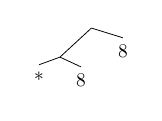
\begin{tikzpicture}[scale=.7] 
       \tikzset{level distance=15pt, sibling distance=10pt}
       \Tree [[  * 8 ] 8 ]
     \end{tikzpicture}
  \end{subfigure}
  \vspace{2mm}

  \hdashrule{.9\linewidth}{1pt}{1pt}


  \vspace{2mm}
  \begin{subfigure}{.17\linewidth}
     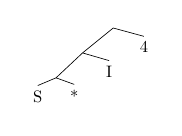
\begin{tikzpicture}[scale=.6] 
       \tikzset{level distance=15pt, sibling distance=10pt}
       \Tree [[[  S * ] I ] 4 ]
     \end{tikzpicture}
     \caption{(16)}
  \end{subfigure}
  \begin{subfigure}{.17\linewidth}
     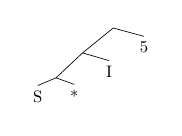
\begin{tikzpicture}[scale=.6]
       \tikzset{level distance=15pt, sibling distance=10pt}
       \Tree [[[  S * ] I ] 5 ]
     \end{tikzpicture}
     \caption{(25)}
  \end{subfigure}
   \begin{subfigure}{.17\linewidth}
     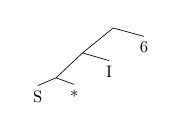
\begin{tikzpicture} [scale=.6]
       \tikzset{level distance=15pt, sibling distance=10pt}
       \Tree [[[  S * ] I ] 6 ]
     \end{tikzpicture}
     \caption{(36)}
  \end{subfigure}
  \begin{subfigure}{.17\linewidth}
     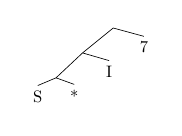
\begin{tikzpicture}[scale=.6] 
       \tikzset{level distance=15pt, sibling distance=10pt}
       \Tree [[[  S * ] I ] 7 ]
     \end{tikzpicture}
     \caption{(49)}
  \end{subfigure}
  \begin{subfigure}{.17\linewidth}
     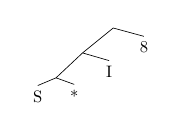
\begin{tikzpicture}[scale=.6] 
       \tikzset{level distance=15pt, sibling distance=10pt}
       \Tree [[[  S * ] I ] 8 ]
     \end{tikzpicture}
     \caption{(64)}
  \end{subfigure}
\end{figure}
\captionsetup[subfigure]{labelformat=parens} 
\vspace{-.3cm}

\noindent The top row consists of one type of representation of an integer
squared, namely, the integer times itself. The bottom row contains
another type of representation in which the function $f(x)=x^2$,
represented in combinatory logic as $S * I$, is applied to the
integer. The top and bottom row of each expression evaluate to the
same integer. If we consider only the first column, the top tree has 4
unique subtrees and the bottom has 7. But each column adds 3 unique
subtrees to the top row and only 2 to the bottom. So by the fifth
column the top row has more unique subtrees than the bottom row. The
increased compressibility of the bottom row is due to the fact that
the squaring operation has been factored out as an abstraction. This
is an example of how this compressibility metric favors
abstraction when multiple expressions are being considered at once.

More sophisticated metrics than the one proposed here exist; we could
use the negative logarithm of the probability of the solutions under a
suitable probability
distribution~\cite{DBLP:journals/tit/BarronRY98}. Future work will
explore whether this sophistication is worthwhile and which prior on
grammars makes sense. For our purposes here, penalizing according to
the number of unique subtrees appropriately and sufficiently rewards
reuse of useful subtrees.

We want to choose a solution for each hit task such that the complete set
of such solutions for all solved tasks is as compressible as
possible. That is, let $t_i$ be a task in the set of hit tasks, and
let $\{e^k_i\}$ be the expressions in the frontier that solve
it. Then our goal is to find
\[
\{e^*_i\} = \argmin_{\{e^k_i\}} | \cup_i e^k_i |,
\]
where $|\cdot|$ denotes the number of unique trees in a set of expressions.

However, an exact optimization of this problem requires examining
$O(M^K)$ assignments, where $M$ is the maximum number of solutions for
any one task, and $K$ is the number of tasks. Since this is
prohibitive, we relax the compressibility metric as follows: we define
the cost of adding each new solution $s_n$ to a partial set of
solutions $s_1, \dots, s_{n-1}$ to be the number of additional unique
subtrees in $s_n$ that are not present in $s_{n-1}$. That is, the
penalty of adding a new expression to the set of expressions depends
only on the last expression we added. Our solution thus becomes
approximate, and that approximation is order-dependent, but a
depth-first search on the defined search space goes from exponential
in the solution degree to quadratic ($O(KM^2)$). 

However, when the number of solutions in the frontier grows, this
quadratic computation becomes prohibitive. Therefore, in practice, we
bound the number of potential expressions we are willing to consider
at any one iteration to any one task to a small number. We find that a
setting of this bound to 2 is computationally feasible and large
enough to guide subcomponent discovery in a reliable way. It may be
necessary to increase this bound as we scale this algorithm to larger
problems.

\subsection{Re-estimating the Stochastic Grammar}

Given a set of chosen solution expressions, which we will call the
\emph{solution set}, want to re-estimate our stochastic grammar. Our
inspiration for doing this is the Nevill-Manning algorithm for
grammar-based compression~\cite{nevill1997identifying}. The idea of
that compression algorithm is to compress any string by creating a
grammar for that string such that a) no two symbols appear more than
once in the grammar and b) every rule is used more than once. From a
set of expressions, we generate a grammar according to these criteria.

%% To do this, we traverse a set of combinator binary trees in
%% depth first order. We count the occurrences of every subtree. Every
%% time we encounter a subtree for the \emph{second} time, we designate
%% it as a primitive in our new grammar. This ensures that every
%% primitive is used more than once. During our traversal, we do not
%% descend into trees that have been added already to the new
%% grammar. Thus, we only count an instance of a tree if that instance is
%% not a subtree of a primitive element of the new grammar.

This procedure generates a parse of the solution set with a new set of
primitives, and we keep count of how many times each primitive
occurred in the solutions set. To estimate the probabilities
associated with each node production, we again traverse the solution
set, but this time for each node we count which other primitive
elements from the new grammar could have been used. In accordance with
Section~\ref{sec:stochgrammar}, we estimate the terminal production weight
to be the ratio of the number of times that node was used in the first
traversal divided by the number of times it was used in the second
traversal.

\section{Experiments.}
\subsection{Symbolic regression.}
\label{sec:symreg}

We first illustrate the performance of our learning algorithm on a
symbolic regression problem. For each task in this problem, we want to
find an algebraic function, symbolically specified, that maps a set of
input values to output values. We choose this problem because it has a
long history in AI, particularly in the genetic programming
literature~\cite{DBLP:books/daglib/0070933}.

In the formulation we consider, each task $t$ corresponds to a
polynomial $f$, and an expression $e$ solves $t$ if it returns the
same value when applied to $i \in 0, \dots, 9$ that $f$ does. In the
experiment shown here, the set of problems corresponds to the set of
all polynomials with degree less than or equal to 2. In the initial
library, we include the basic combinators I, S, B, C and four
arithmetic primitives $1$, $0$, $*$, and $+$. The choice of initial
weights on these primitives can make a difference, as it determines
the relative ordering of combinators in the enumeration step. To get a
general sense of the algorithm's performance, we set the initial
weights to be slightly different on each run, perturbing them around a
uniform weighting.

\setcounter{subfigure}{0} 
\begin{figure}[ht]
\centering
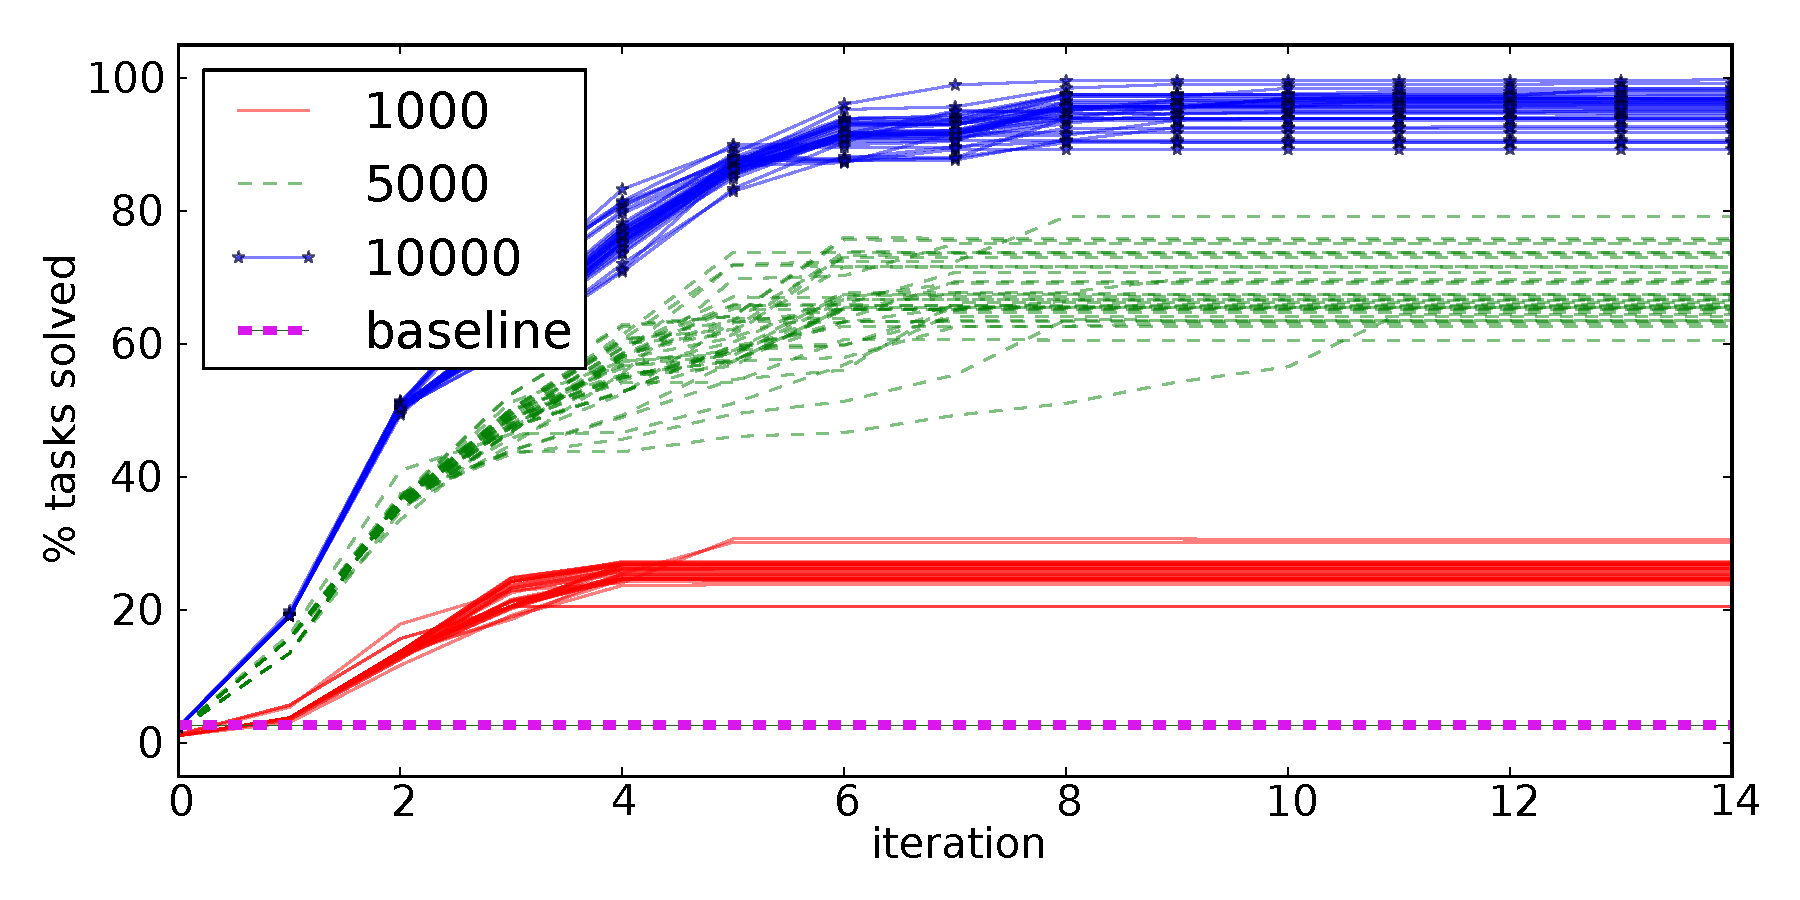
\includegraphics[width=1.0\linewidth]{figures/symreg3frontiers.pdf}
\caption{Learning curves as a function of frontier size.  As frontier
  size is increased, curves plateau closer to $100\%$ performance. A
  baseline search over $150000$ expressions only hits $3\%$ of the
  tasks (dashed pink line). \label{fig:symregLearning}}
\end{figure}
\begin{figure}[ht]
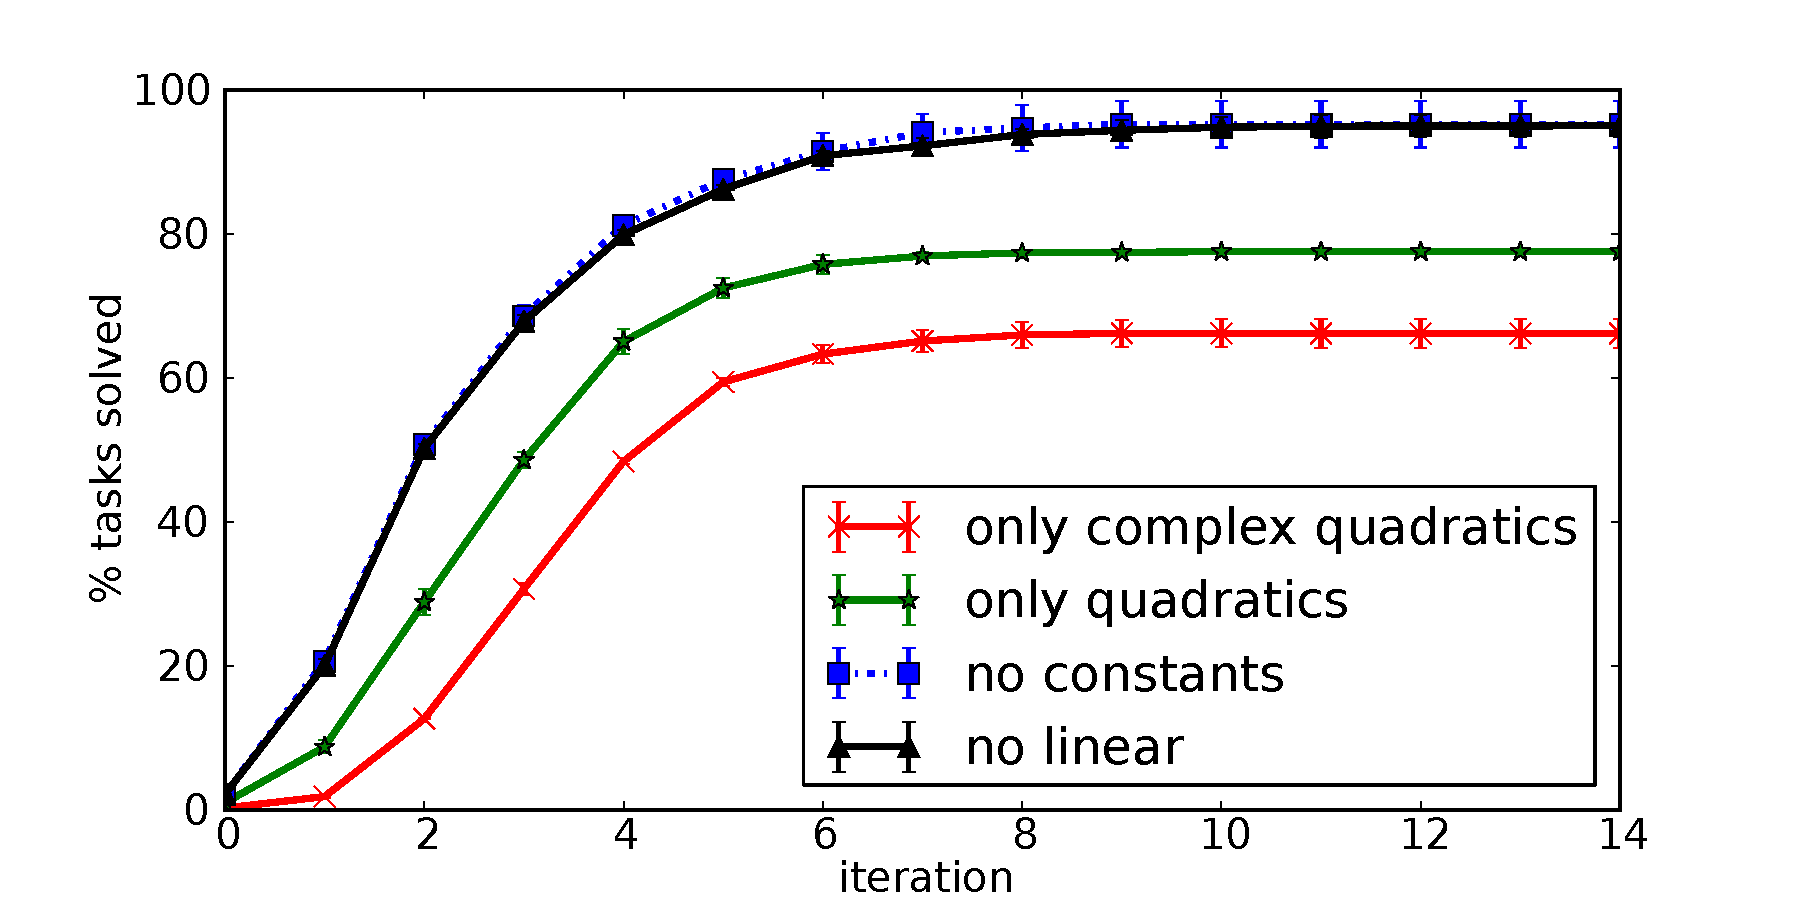
\includegraphics[width=1.07\linewidth]{figures/symRegDiffCurricula.pdf}
\caption{How do different task sets affect learning curves? Learning
  curves at a frontier size of $10000$ for different task
  sets.} 
\label{fig:symregCurricula}

\end{figure}




%% Why do the learning curves asymptote early? One might object that a
%% learning algorithm should continuously improve, if only slowly, as it
%% is given more time. But in these runs we observe a finite and
%% permanent performance cap. This is expected: once the learner find a
%% set of concepts it can explain, if those concepts fill up the
%% frontier, then there is nothing to spur the learner to incorporate as
%% yet unsolved tasks. 

%% To investigate whether this is in fact the case, we can examine the
%% proportion of expressions in the frontier that match tasks in our task
%% set; that is, is the learning curve plateauing because the frontier is
%% heavily redundant, or is it plateuing because the frontier contains
%% many expressions that do not hit the task set at
%% all? Figure~\ref{fig:plateau_investigation} shows the proportion of
%% the expressions in the frontier that hit a task as the frontier size increases.


In Figure~\ref{fig:symregLearning}, we show performance results as we
vary the frontier size. Changing the frontier size changes the number
of tasks the algorithm identifies correctly over the course of 15
algorithm iterations (all experiments in this work were run for 15
iterations). As a baseline, we enumerated $10000*15=150000$
expressions from the initial grammar. This is the total number of
expressions that a run of the algorithm sees if it has a frontier size
of $10000$ and runs for $15$ iterations. Thus, if the benefit accruing
to the runs with larger frontier sizes is simply due to an increase in
the number of expressions seen, rather than increased learning, we
should see similarly good performance from this baseline run. In fact,
however, the baseline run only hits $27$ of the $1000$ tasks ($3\%$),
whereas our algorithm nears $100\%$ for a frontier of $10000$.

What does the E.C. algorithm learn in this task?  Inspecting the top
weighted primitives of the final grammars, we find many incrementers
(e.g. (+1), (+2), etc.), several versions of expressions that
translate to functions like $x*f(x)$ and $f(x*f(x))$, and combinations
of these, like $x*(x+3)+3$ and $x*(x+2)$. Informally, we see
expressions that apply functions to themselves, building up complex
functions with relatively few unique primitives. 

To what degree is ``conceptual bootstrapping'' responsible for the
improved performance. That is, to what extent does the presence of
simple problems account for the ability to learn complex functions?
One hypothesis is that to succeed on a set of tasks, the set must
contain a ``learnable'' curriculum, a set of tasks that serve as
stepping stones from an impoverished representation to a rich one. We
can test this hypothesis by varying the set of tasks to which the E.C.
algorithm is exposed. If it is true, then we should see a nonlinear
response to reducing the number of easy tasks, as the curriculum
changes from being learnable to being unlearnable.

In Figure~\ref{fig:symregCurricula}, we present learning curves
(frontier size~10000) corresponding to various versions of our
original symbolic regression task set. Recall that the original set
consisted of all polynomials of degree two or less and with
coefficients between 0 and 9. In the ``no constant'' task set, we
remove the 9 constant functions in this set. In the ``no linear'' task
set, we remove 90 linear functions from the set. We observe that
performance on those task sets does not decrease. However, when we
remove both the linear functions and the constant function (``only
quadratics''), we see a sharp drop in the algorithm's
performance. When we further restrict the task set to only ``complex''
quadratics (which we define as quadratics whose
coefficients are greater than zero), we observe another comparable
drop in performance. When we go one step further and restrict the task
set to quadratics with coefficients greater than 1, performance drops
to 0 because no task is hit in the initial frontier. 

This data has in it the nonlinearity that we predicted -- that a
minimal curriculum of simple tasks is sufficient to achieve high
performance -- but also suggests that, at least in this domain, this
is not an all-or-none effect. Though the performance drops
significantly once no linear functions are included in the task set,
learning does still occur, and the learning curves still have the same
basic shape. 

%% In addition, we have a
%% baseline for each curve, visits the same number of expressions as the
%% corresponding algorithm run (i.e. frontier size $\times$ $\#$ of
%% iterations) but all at once; it does not do any learning. Thus, this
%% baseline serves as a brute-force control for the learning aspect of
%% the algorithm.


\subsection{Boolean Function Learning}
\label{sec:boolcircuits}

\begin{figure}[t]
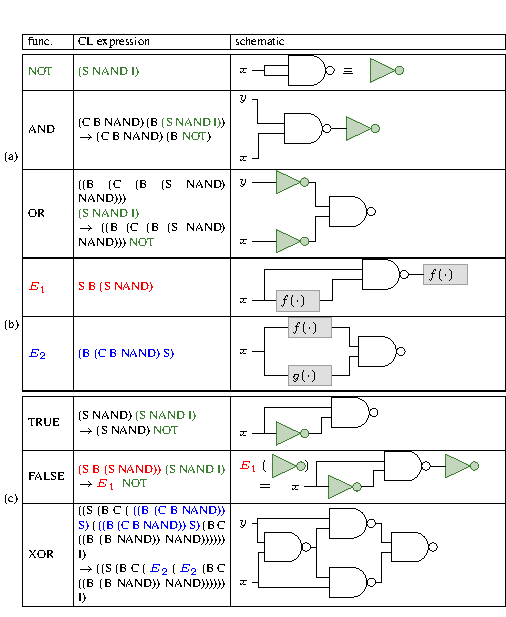
\includegraphics{./figures/tablealonedoc.pdf}
\caption{Some learned primitives from the circuit based Boolean
  function learning experiment. We highlight compression using $NOT$,
  $E_1$ and $E_2$. \,(a) The three elementary gates used to generate
  the task set. (b) Two higher-order primitives in the induced
  grammar. Note how $E_1$ can be used to define FALSE by taking the
  NOT function as an argument. (c) Additional common Boolean functions
  found in the learned grammar.  \label{table:booleanCircuits}}
\end{figure}



As another demonstration of our approach, we investigate the
E.C. algorithm's ability to learn Boolean functions using only the logical
primitive NAND and the basic combinators. It is well known that a
Boolean circuit can be constructed for any Boolean function given only
the NAND gate. Here, the basic combinators take the place of the
wiring normally found in a circuit.

We constructed two task sets. The first of these was constructed
explicitly to contain familiar modular structure. In this set of
tasks, we sampled $1000$ Boolean circuits using AND, OR, and NOT
gates. To accomplish this, we first sampled either 1, 2 or 3 inputs,
then between 1 and 5 gates, randomly wiring the inputs of each new
gate to the output of one of the existing gates in the circuit. We
continued this sampling procedure until we had 1000 ``connected''
circuits, i.e., circuits all of whose outputs are wired to an input
except for the last one (the output gate). This resulted in $1000$
tasks consisting of $82$ unique Boolean functions, with a distribution
of tasks as shown in Figure~\ref{fig:booldistr}a. In
Figure~\ref{fig:boolLearningCurvesCircuits}, we present learning
curves for frontier sizes 100, 500 and 10000, using the same procedure
as in Section~\ref{sec:symreg}. In Figure~\ref{fig:booldistr}, we show
that the distribution over Boolean functions enumerated from the
grammar over expressions is much more similar to the true function
distribution after learning than before.

\begin{figure}
\vspace{.5cm}
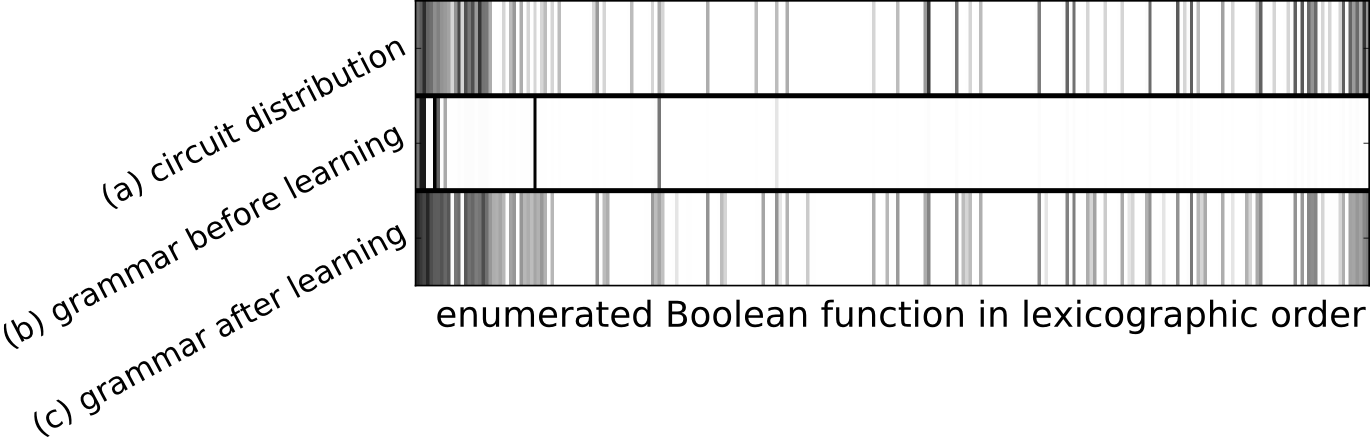
\includegraphics[width=\linewidth]{figures/circuitDistrComp2.png}
\caption{Distribution of Boolean functions among (a) the set of 1000
  circuits randomly constructed from AND, OR and NOT gates (see text);
  b) the first 1000 expressions from the grammar over expressions
  \emph{before} learning; c) the first 1000 expressions from the
  grammar over expressions \emph{after} learning. Gray levels indicate
  percent of instances (circuits/expressions) which evaluate to that
  function. Functions increase in domain size from left to right; each
  function can be represented as a binary string corresponding to the
  output column of the truth table, and functions are ordered with
  respect to these strings. \label{fig:booldistr}}
\end{figure}

This problem is particularly suitable for inspecting the constituents
of the induced grammar $\mathcal{G}$. We might hope that our algorithm
recovers the constituent logic gates that were used to build up the
tasks. Table~\ref{table:booleanCircuits} shows a few of the top ranked
expressions in the library. These include the basic logic gates; we
also include two higher-order expression $E_1$ and $E_2$, to stress
that the representation the E.C. algorithm is using allows it to build
concepts that are more expressive that just sub-circuits.

In a second experiment, we include all $272$ Boolean truth tables with
three or fewer inputs as tasks. This is a more difficult
problem. There are two kinds of learning that the E.C. algorithm might
accomplish: first, many expressions in $\mathcal{L}$ map to a single
Boolean function, so it needs to learn primitives that allow it to
span many different functions instead of generating very simple
functions redundantly. The second kind of learning involves the
distribution of the functions themselves. In the circuit based Boolean
experiment, that structure is apparent in the distribution in
Figure~\ref{fig:booldistr}. In this second experiment, we remove the
second kind of structure. In
Figure~\ref{fig:boolLearningCurvesUniform}, we show 10 runs of the
E.C.  algorithm on the second experiment with a frontier size of
$2000$: note how there are several local minima that the majority of
the runs get stuck in with performance around $50\%$, but several of
the runs seem to take different trajectories to more successful
representations.

\vspace{-.3cm}
\begin{figure}[h]
\begin{subfigure}{.1\linewidth}
\caption{\label{fig:boolLearningCurvesCircuits} }
\end{subfigure}
\begin{subfigure}[Before]{0.9\linewidth}
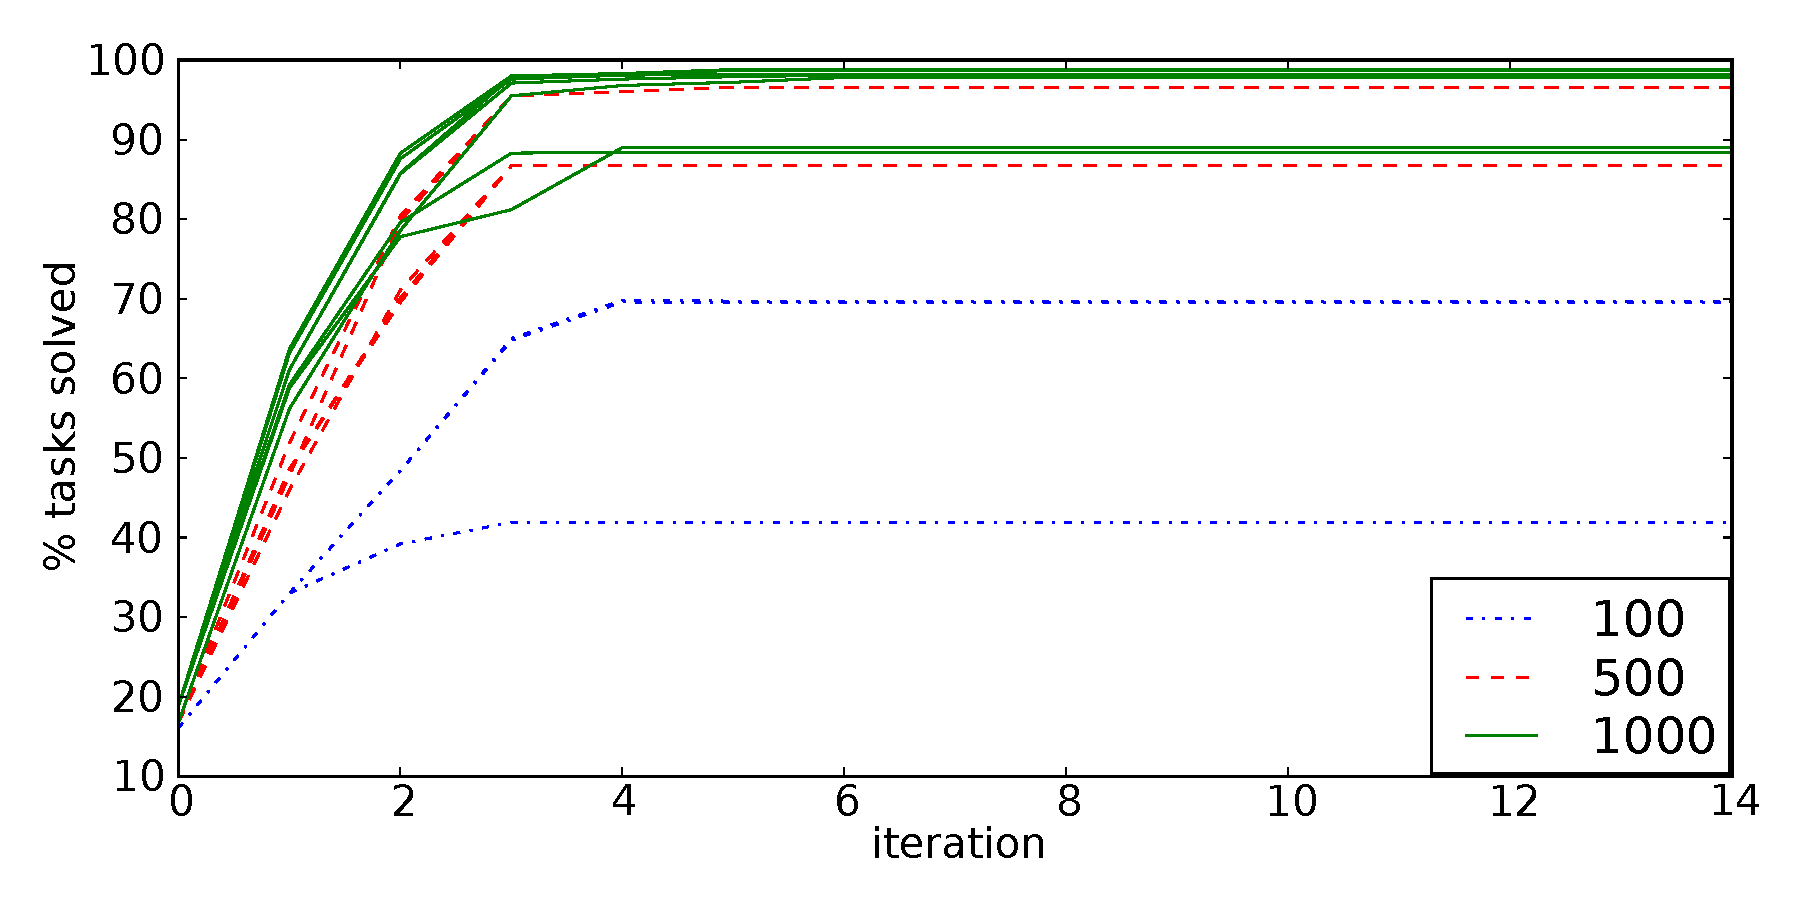
\includegraphics[width=1.0\linewidth]{figures/booleancircuits3frontiers.pdf}
\end{subfigure}

\vspace{-.32cm}
\begin{subfigure}{.1\linewidth}
\caption{\label{fig:boolLearningCurvesUniform}}
\end{subfigure}
\begin{subfigure}[After]{.9\linewidth}
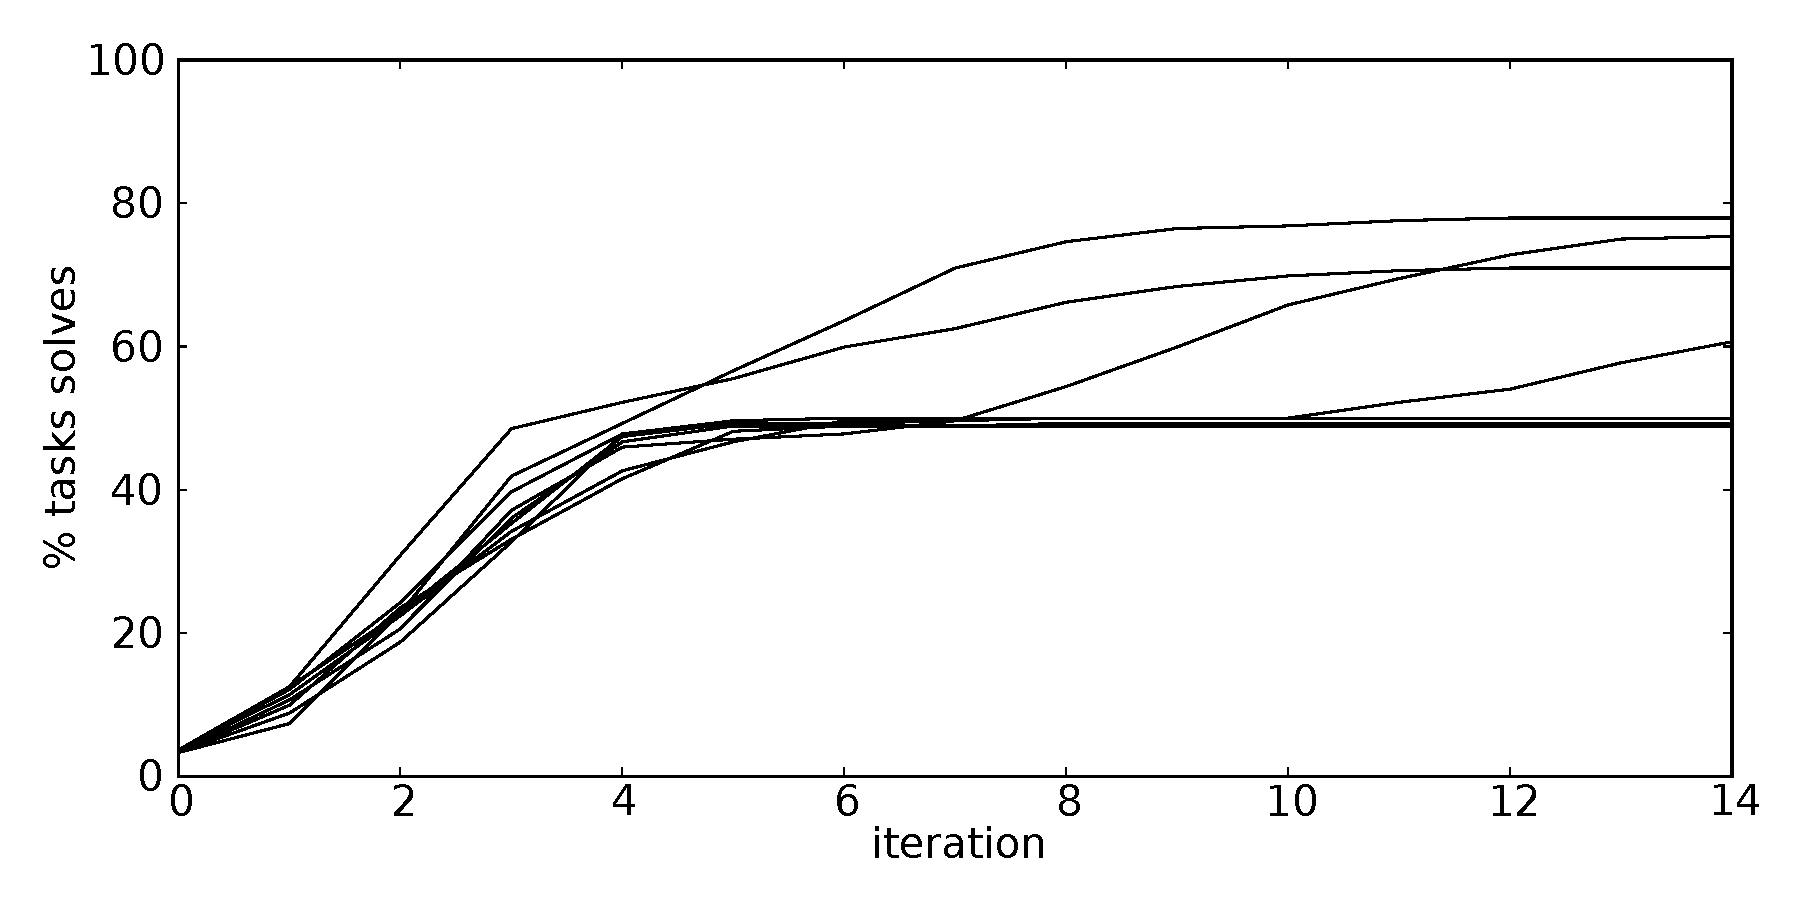
\includegraphics[width=1.0\linewidth]{figures/booleanfunctionsUniform.pdf}

\end{subfigure}
\caption{Learning curves from Boolean function learning
  experiments. (a) Learning curves for various frontier sizes on task
  set of circuit based Boolean functions. (b) 10
  learning curves for frontier size of 2000 on a task set consisting
  of all Boolean functions of cardinality 3 or smaller. Note how most
  of the trajectories get stuck in a local minimum around
  $50\%$.\label{fig:boolLearningCurves}}
\end{figure}

\section{Conclusion}
This work brings together ideas from various areas of research --
hierarchical Bayes, learning to learn, minimum description length
learning, and learning programs -- to provide a proof of concept for
how bootstrap learning of abstract composable concepts can rapidly
facilitate problem solving in the absence of domain specific
knowledge. We show that this approach can learn successfully even in
domains for which the solution space is not smooth and the error
signal is all or none, where the only sense of locality to guide
learning is the modular and compositional structure of the solutions
that the algorithm itself builds.

The problem presented here was chosen to highlight the vastness of the
search space confronting an agent with minimal background knowledge:
the reward function is binary, it is deterministic, and it cannot
provide feedback about partial solutions. In ongoing work we are
exploring a more probabilistic version of the algorithm that can take
into account continuous rewards, noisy data, and partial solutions.

Our specific implementation of this approach involved a number of
choices which should be explored further in future work.  Our claim
here is not that the E.C. algorithm is optimal, but that it captures key
features of how people solve the problem of learning new systems of
concepts in acquiring deep domain expertise.  Much like a human
researcher investigating a new area of study, our algorithm tries
different models, watches them fail or succeed, and abstracts out the
model elements that capture relevant differences.  It recombines and
reuses successful patterns of reasoning that span many problems in a
domain.

At their best, human processes of discovery clearly go beyond
what our algorithm is capable of.  The algorithm can get stuck in
plateaus after a rapid initial increase in performance, due to its
circular nature: it only inspects the region of the solution space
that is typical of solutions already found.  Humans can become stuck
in similar ways, but at least sometimes they realize that they are
stuck and attempt to find another class of concepts for the remaining
unsolved tasks.  Our algorithm requires, as human learners do, a
sufficiently graded ``curriculum'', or spectrum of problems to solve --
simple problems provide necessary stepping stones to building complex
representations.  Also like humans, our algorithm can adaptively
``self-pace'' its ways through the curriculum, figuring out which
problems it is ready to tackle when, which problems are appropriately
difficult given what it currently knows.  Yet people can sometimes
more intelligently compose and modify the set of problems under
consideration, designing their own stepping stones to expand the set
of problems they can solve.  Making bootstrap learning systems smarter
in these more human-like ways is a prime target for future research.


%% The file named.bst is a bibliography style file for BibTeX 0.99c
\bibliographystyle{named}
\bibliography{Dechter.IJCAI13.CameraReady}
%% \nocite{*}

\end{document}

